%% 
%% Copyright 2007, 2008, 2009 Elsevier Ltd
%% 
%% This file is part of the 'Elsarticle Bundle'.
%% ---------------------------------------------
%% 
%% It may be distributed under the conditions of the LaTeX Project Public
%% License, either version 1.2 of this license or (at your option) any
%% later version.  The latest version of this license is in
%%    http://www.latex-project.org/lppl.txt
%% and version 1.2 or later is part of all distributions of LaTeX
%% version 1999/12/01 or later.
%% 
%% The list of all files belonging to the 'Elsarticle Bundle' is
%% given in the file `manifest.txt'.
%% 

%% Template article for Elsevier's document class `elsarticle'
%% with numbered style bibliographic references
%% SP 2008/03/01

\documentclass[preprint,1p]{elsarticle}
\biboptions{numbers,sort&compress}

%% Use the option review to obtain double line spacing
%% \documentclass[authoryear,preprint,review,12pt]{elsarticle}

%% Use the options 1p,twocolumn; 3p; 3p,twocolumn; 5p; or 5p,twocolumn
%% for a journal layout:
%% \documentclass[final,1p,times]{elsarticle}
%% \documentclass[final,1p,times,twocolumn]{elsarticle}
%% \documentclass[final,3p,times]{elsarticle}
%% \documentclass[final,3p,times,twocolumn]{elsarticle}
%% \documentclass[final,5p,times]{elsarticle}
%% \documentclass[final,5p,times,twocolumn]{elsarticle}

%% For including figures, graphicx.sty has been loaded in
%% elsarticle.cls. If you prefer to use the old commands
%% please give \usepackage{epsfig}

%% The amssymb package provides various useful mathematical symbols
\usepackage{amssymb}
\usepackage{lineno}
\usepackage{hyperref}
\usepackage{siunitx}
\usepackage{multirow}
\usepackage{wasysym}
%\usepackage[percent]{overpic}
%\usepackage[usenames,dvipsnames,svgnames,table]{xcolor}
%\usepackage{cleveref}

%% The amsthm package provides extended theorem environments
%% \usepackage{amsthm}

%% The lineno packages adds line numbers. Start line numbering with
%% \begin{linenumbers}, end it with \end{linenumbers}. Or switch it on
%% for the whole article with \linenumbers.
%% \usepackage{lineno}

\journal{Nucl. Instrum. Meth. A}

\begin{document}

\linenumbers

\begin{frontmatter}

%% Title, authors and addresses

%% use the tnoteref command within \title for footnotes;
%% use the tnotetext command for theassociated footnote;
%% use the fnref command within \author or \address for footnotes;
%% use the fntext command for theassociated footnote;
%% use the corref command within \author for corresponding author footnotes;
%% use the cortext command for theassociated footnote;
%% use the ead command for the email address,
%% and the form \ead[url] for the home page:
%% \title{Title\tnoteref{label1}}
%% \tnotetext[label1]{}
%% \author{Name\corref{cor1}\fnref{label2}}
%% \ead{email address}
%% \ead[url]{home page}
%% \fntext[label2]{}
%% \cortext[cor1]{}
%% \address{Address\fnref{label3}}
%% \fntext[label3]{}

\title{Studies of FBK UFSD3 low-gain avalanche detectors}

%% use optional labels to link authors explicitly to addresses:
%% \author[label1,label2]{}
%% \address[label1]{}
%% \address[label2]{}

\author[1]{A.~Apresyan\corref{cor}}\ead{apresyan@fnal.gov}
\author[5,7]{R.~Arcidiacono}
\author[5]{N.~Cartiglia}
\author[8]{M.~Carulla}
\author[2]{O.~Cerri}
\author[1]{G.~Derylo}
\author[5]{M.~Ferrero}
\author[8]{D.~Flores}
\author[9]{A.~Ghassemi}
\author[3]{H.~Al Ghoul}
\author[1]{R.~Heller}
\author[8]{S.~Hidalgo}
\author[1]{M.~Hussain}
\author[9]{S.~Kamada}
\author[1]{S.~Los}
\author[5]{M.~Mandurrino}
\author[8]{A.~Merlos}
\author[3]{N.~Minafra}
\author[4]{A.~Ovcharova}
\author[8]{G.~Pellegrini}
\author[1,2]{C.~Pena}
\author[8]{D.~Quirion}
\author[3]{C.~Royon}
\author[5]{V.~Sola}
\author[2]{M.~Spiropulu}
\author[5]{A.~Staiano}
\author[1]{L.~Uplegger}
\author[2]{S.~Xie}

\address[1]{Fermi National Accelerator Laboratory, Batavia, IL, USA}
\address[2]{California Institute of Technology, Pasadena, CA, USA}
\address[3]{University of Kansas, KS, USA}
\address[4]{University of California Santa Barabara, CA, USA}
\address[5]{INFN, Torino, Italy}
\address[6]{Universit\`a di Torino, Torino, Italy}
\address[7]{Universit\`a del Piemonte Orientale, Italy}
\address[8]{Centro Nacional de Microelectr\'{o}nica (IMB-CNM-CSIC), Barcelona, Spain}
\cortext[cor]{Corresponding author}

\begin{abstract}
%% Text of abstract
abstract
\end{abstract}

\begin{keyword}
%% keywords here, in the form: keyword \sep keyword

%% PACS codes here, in the form: \PACS code \sep code
Silicon \sep Timing \sep LGAD \sep Test Beam
%% MSC codes here, in the form: \MSC code \sep code
%% or \MSC[2008] code \sep code (2000 is the default)

\end{keyword}

\end{frontmatter}

\tableofcontents

%% \linenumbers

%% main text
\section{Introduction} 

Future colliders, including the high luminosity upgrade of the Large Hadron
Collider (HL-LHC) at CERN, will operate with instantaneous luminosity an order of magnitude higher than what has been achieved at the
Large Hadron Collider (LHC) so far.
With the increased instantaneous luminosity, the rate of simultaneous
interactions per bunch crossing (pileup) is projected to reach an average of 140
to 200. The large amount of pileup exacerbates the difficulties in separating 
particles from the hard scattering interaction with those
produced in pileup interactions. In particular, the ability to discriminate between
jets produced in the events of interests, especially those associated with vector 
boson fusion processes, and jets produced by pileup interactions will be
degraded. Additionally, the efficiency to identify high $p_{\mathrm{T}}$ isolated electrons
and muons will be severely reduced due to the high density of pileup particles
in their vicinity. The missing transverse energy resolution will also deteriorate, and several
other physics objects performance metrics will also suffer the
detrimental effects of pileup.


One way to mitigate the pileup effects mentioned above, complementary to
precision tracking methods, is to measure a time of arrival 
associated with each particle. Such a measurement with a precision of about
30-40~\si{ps}, will reduce the effective amount of pileup by a factor of 10,
given that the spread in collision time of the pileup interactions at HL-LHC is
foreseen to be approximately 200~\si{ps}. It has been previously shown that a
precision of better than $20$~\si{ps} can be achieved for electromagnetic
showers measured with silicon sampling
calorimeters~\cite{Apresyan201662,Apresyan2017_NSSMIC,AKCHURIN201731} using
traditional planar silicon detectors. In this paper, we report results of
particle beam measurements with thin low-gain avalanche detectors (LGAD) that
have been shown to achieve time resolutions around
30~\si{ps}~\cite{Cartiglia201783, PELLEGRINI201412}. LGAD are envisioned to be
used in the CMS and ATLAS experiment upgrades for HL-LHC in order to overcome
the event reconstruction challenges posed by the high rate of concurrent
collisions per beam crossing. The implemented regions of pseudorapidity ($\eta$)
are: $1.6 < |\eta| < 2.9$, and $2.4 < |\eta| < 4.2 $ for CMS and ATLAS, respectively. In
order to achieve the desired timing precision over the entire surface area of the
detectors, the sensors will need to provide high uniformity of signal response. In this paper, we perform detailed measurements of the
performance of LGAD sensors produced by Fondazione Bruno Kessler exposed to the 120~GeV proton beam at
Fermilab. Utilizing high-precision tracking detectors we extract position
dependence of the charged-particle detection efficiency, signal pulse height,
signal timestamp, and time resolution of 50~$\mu$m LGAD sensors. We also study the time resolution of FBK sensors irradiated to an equivalent neutron fluence of $1.5\times 10^{15}$~n/cm$^2$. Detailed measurements of irradiated HPK sensors were presented in Ref.~\cite{Galloway:2017gfx}.

The paper is organized as follows: the tested LGAD sensors and
their operating conditions are discussed in Sec.~\ref{sec:sensors};
the experimental setup and data analysis
procedures are described in Sec.~\ref{sec:setup}; 
studies of sensor irradiation tolerance are presented in 
Sec.~\ref{sec:irradiationStudies}; studies of large area sensors are presented 
in Sec.~\ref{sec:largeAreaStudies}; and the conclusion is given in Sec.~\ref{sec:conclusion}.


\section{LGAD Sensors}
\label{sec:sensors}

% Describe UFSD3 and UFSD2 sensor productions
% What's new with respect to previous productions? 
% expected features?

Sensors from two recent FBK productions were studied in this test beam. The latest production, Ultra-Fast Silicon Detectors 3 (UFSD3) features an innovative technique: the addition of carbon doping, which is expected to mitigate radiation damage to the gain layer and extend the life of the sensors.
This test beam focused on carbonated sensors in 1x2 arrays of 1x3mm pads, prepared with irradiations of \num{5e14}~neq and \num{1.5e15}~neq. The performance of the irradiated sensors is compared with that of their unirradiated counterpart to evaluate the effectiveness of the carbon dose for improving the radiation hardness.

Additionally, the development of a 16-channel LGAD readout board at Fermilab has facilitated the systematic study of larger arrays in a test beam for the first time. Demonstrating the feasibility of producing large sensors with highly uniform signals is a critical step towards building a large area detector with good timing performance. In this test beam, a 2x8 array of 2x2~mm$^{2}$ pads from UFSD2, the previous FBK LGAD production, was studied and evaluated for uniformity. Photos of the 2x8 array and the 16-channel readout board can be seen in Fig.~\ref{fig:array_photo}.


\begin{figure}[htp] 
\centering 
\begin{tabular}{c} 
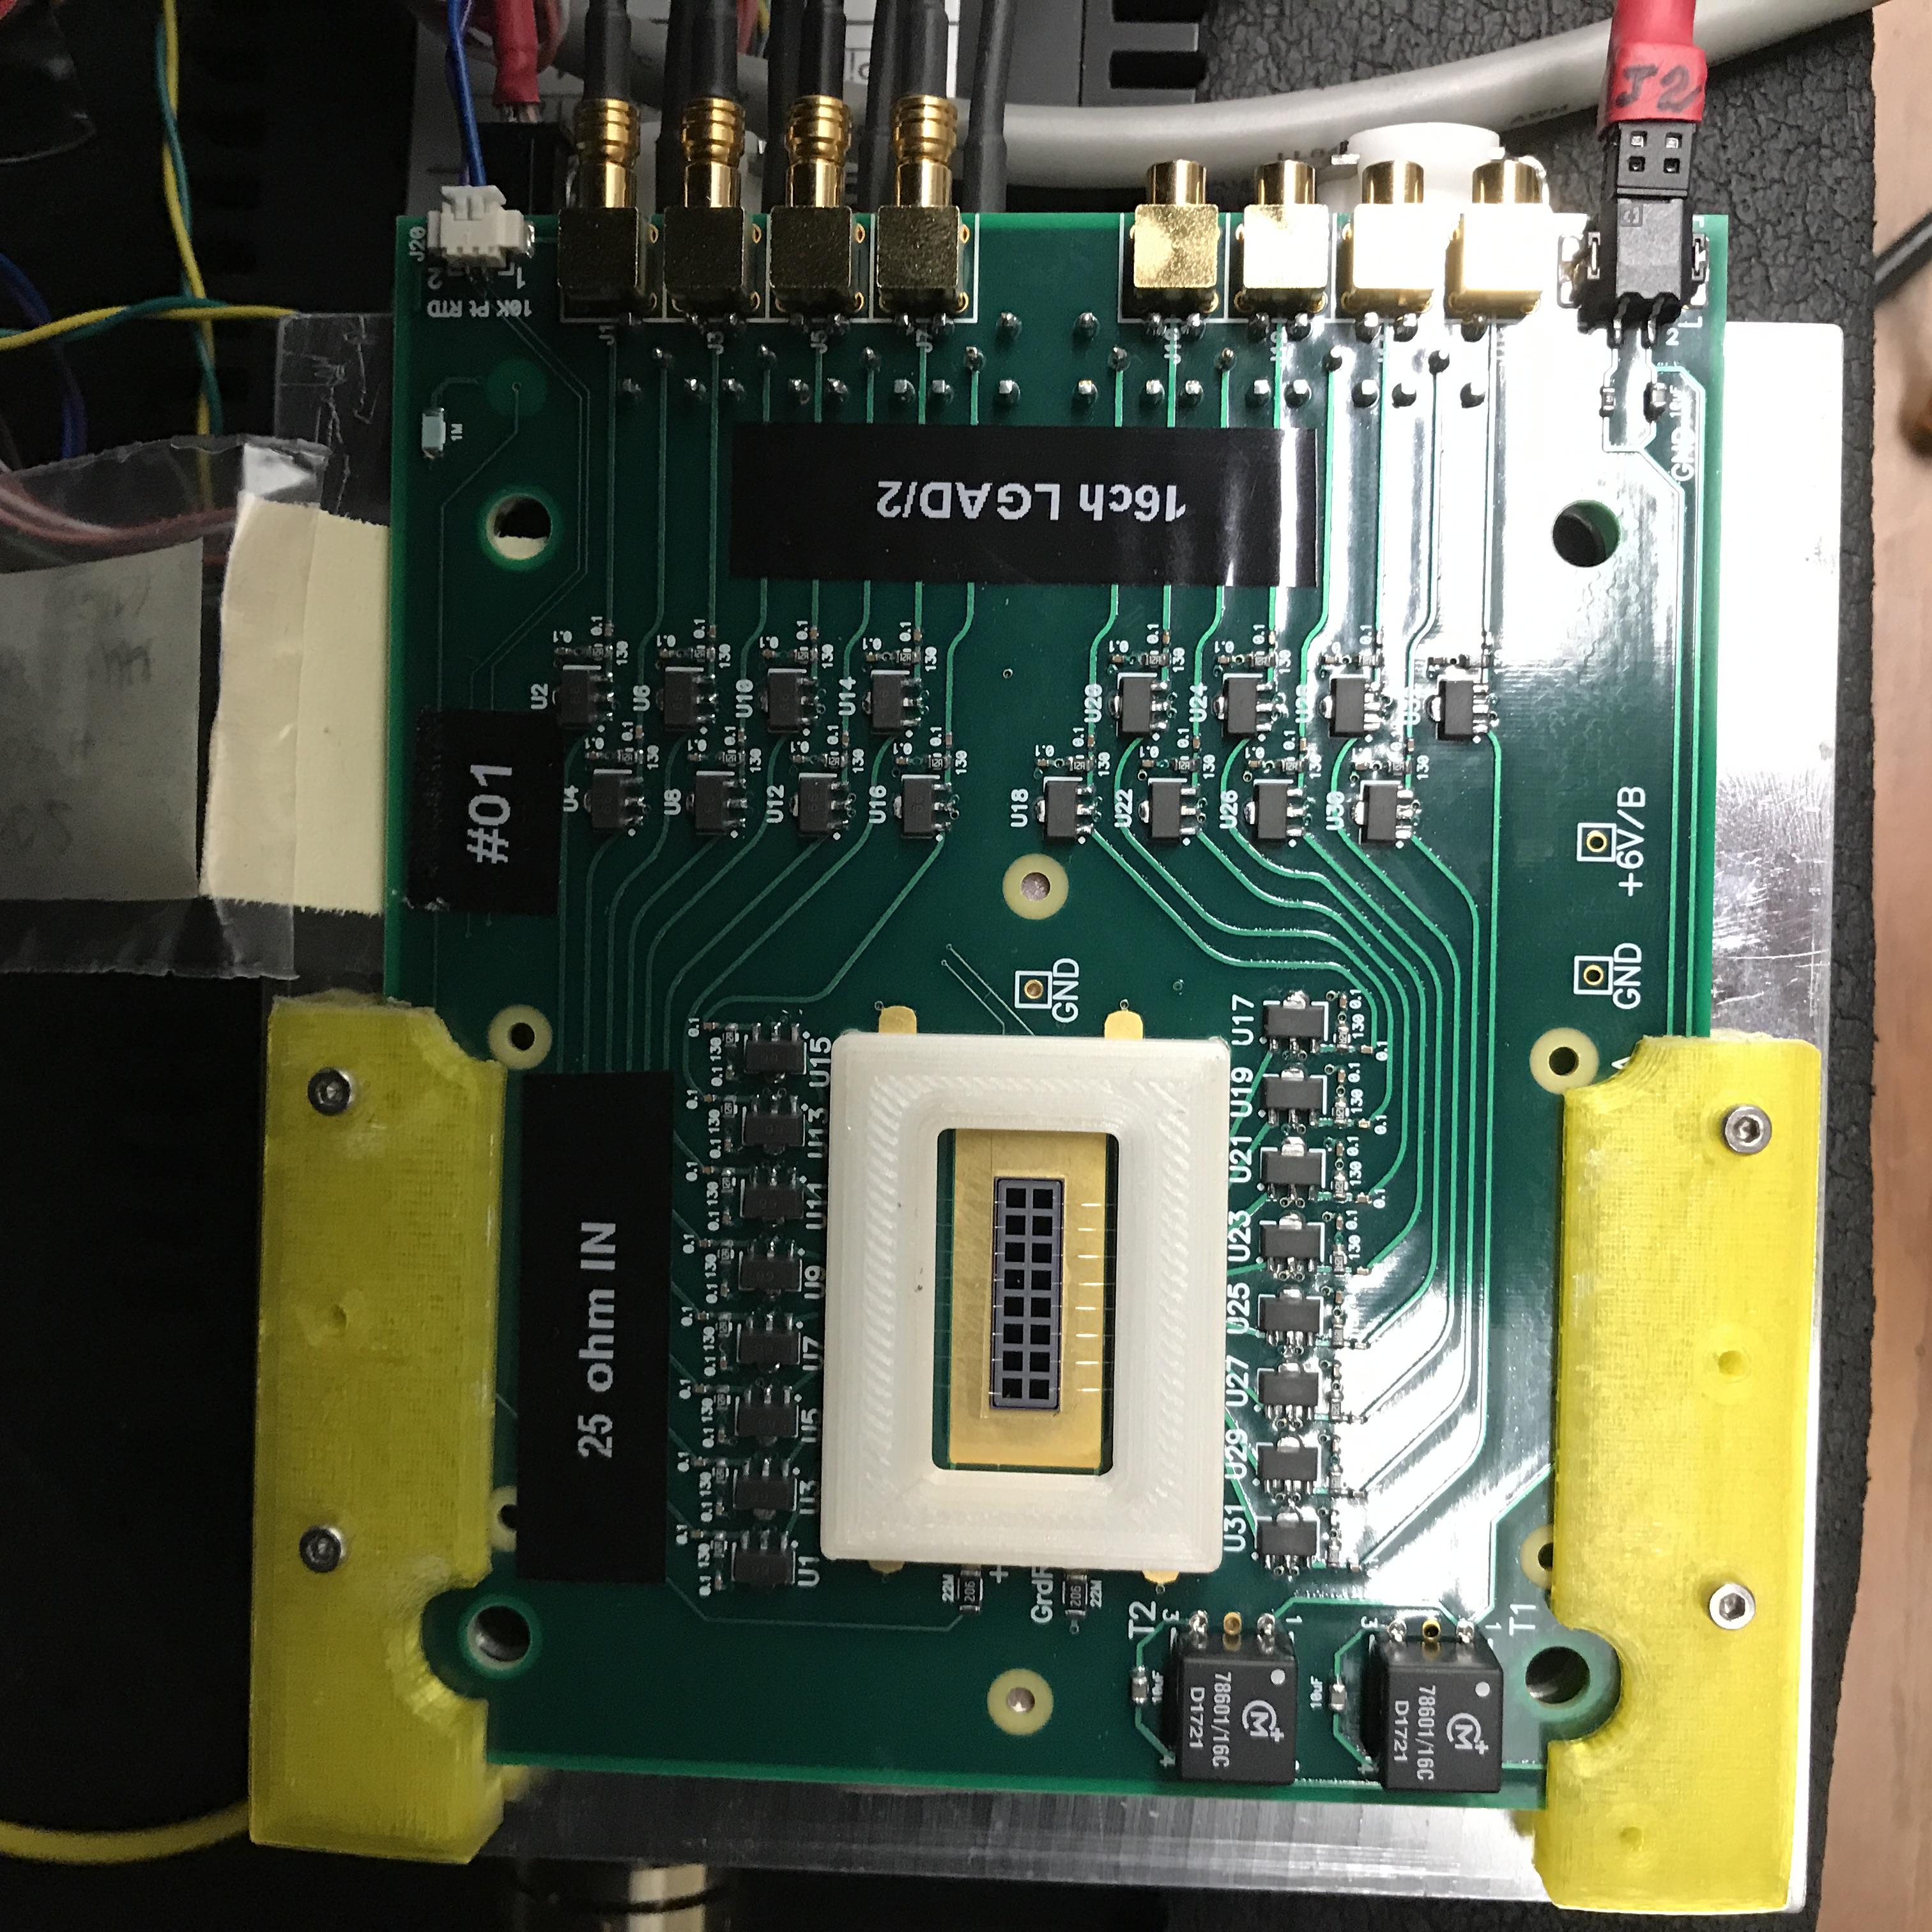
\includegraphics[width=0.8\textwidth]{fig/arrayphoto}   

\end{tabular} 
\caption{Replace with better photo of sensor and board. Add photo of W5 sensor}
\label{fig:array_photo} 
\end{figure} 


\section{Experimental Setup and Data Analysis} 
\label{sec:setup}
\subsection{Fermilab Test-beam Facility}
%FTBF facility
%Readout electronics%
%Brief description of analysis selection and reconstruction algorithms
Test-beam measurements were performed at the Fermilab Test-beam Facility (FTBF)
which provided a $120$~GeV proton beam from the Fermilab Main Injector
accelerator. 

The Devices Under Test (DUTs) were mounted on a remotely operated
motorized stage inside a cold, dry, and dark box. The cold box was placed behind the FTBF pixel telescope detector~\cite{KWAN2016162}, which provides better than 10~$\mu$m position resolution for charged
particles impinging on the DUT. Additionally, a Photek~240 micro-channel plate
(MCP-PMT) detector~\cite{Anderson:2015gha, MCPFastCaloNIMA,
Ronzhin2015288,Ronzhin201552} was placed inside the cold box, next to the LGADs and provided a very precise reference timestamp. Its precision has been previously 
measured to be less than $7$~ps~\cite{Ronzhin2015288}. A schematic diagram and
photograph of the experimental area are shown in Fig.~\ref{fig:DragonBoxDiagram}
and Fig.~\ref{fig:DragonBox}, respectively. 

Two DAQ systems are used to acquire signals from the DUTs. For precise time resolution measurements, a \SI{2.5}{\giga\Hz} 4-channel Tektronix scope is used with 14-bit resolution and a sampling rate of 10 GS/s.
For many-channel measurements, a 32-channel CAEN V1742 digitizer board~\cite{CAENDRS} is used, which provides digitized waveforms sampled at 5 GS/s, with one ADC count corresponding to approximately 0.5~mV. The CAEN digitizer was
voltage- and time-calibrated using the procedure described in
Ref.~\cite{Kim201467}. One of the main parameters of DAQ system for precise time
measurements is the ``electronic time resolution'', defined as the measured time
jitter between two signals that are split from the same source. These two
signals are used as ``start'' and ``stop'' signals to electronic system
measuring the time interval between them. The electronic time resolution of the
CAEN V1742 digitizer was measured to be less than 4~ps, and thus, its impact on
the timing measurements presented in these studies can be neglected. The DAQ for
the pixel telescope is based on the CAPTAN system developed at
Fermilab~\cite{KWAN2016162}. The track-reconstruction is performed using the
Monicelli software package developed specifically for the test-beam application. 

\begin{figure}[htbp] 
\centering
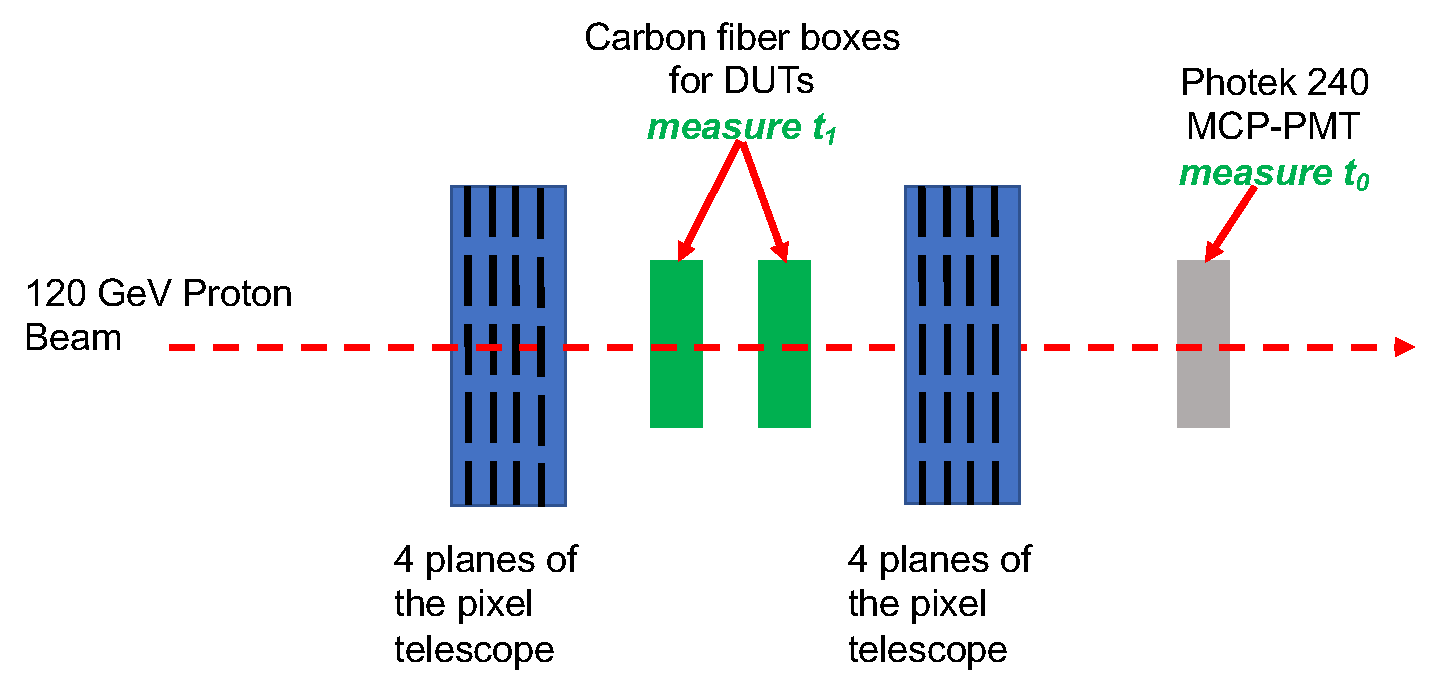
\includegraphics[width=0.75\textwidth]{fig/BeamSetup.pdf} 
\caption{REPLACE. A schematic diagram of the test-beam setup is shown. The $t_0$ and $t_1$ are defined in Section 4.} 
\label{fig:DragonBoxDiagram} 
\end{figure} 

The coldbox housing the DUTs contains stages that can be controlled remotely to move the sensors in the horizontal and vertical directions in order to align them with the beam. 
The readout boards hosting the sensors are mounted on aluminum blocks with channels hollowed out for the passage of cooling fluid. The blocks are connected to a chiller circulating ethylene glycol operating at \SI{-30}{\celsius}. The sensors reach approximately \SI{-18}{\celsius}, as measured by on-board thermistors.

\begin{figure}[htbp] 
\centering
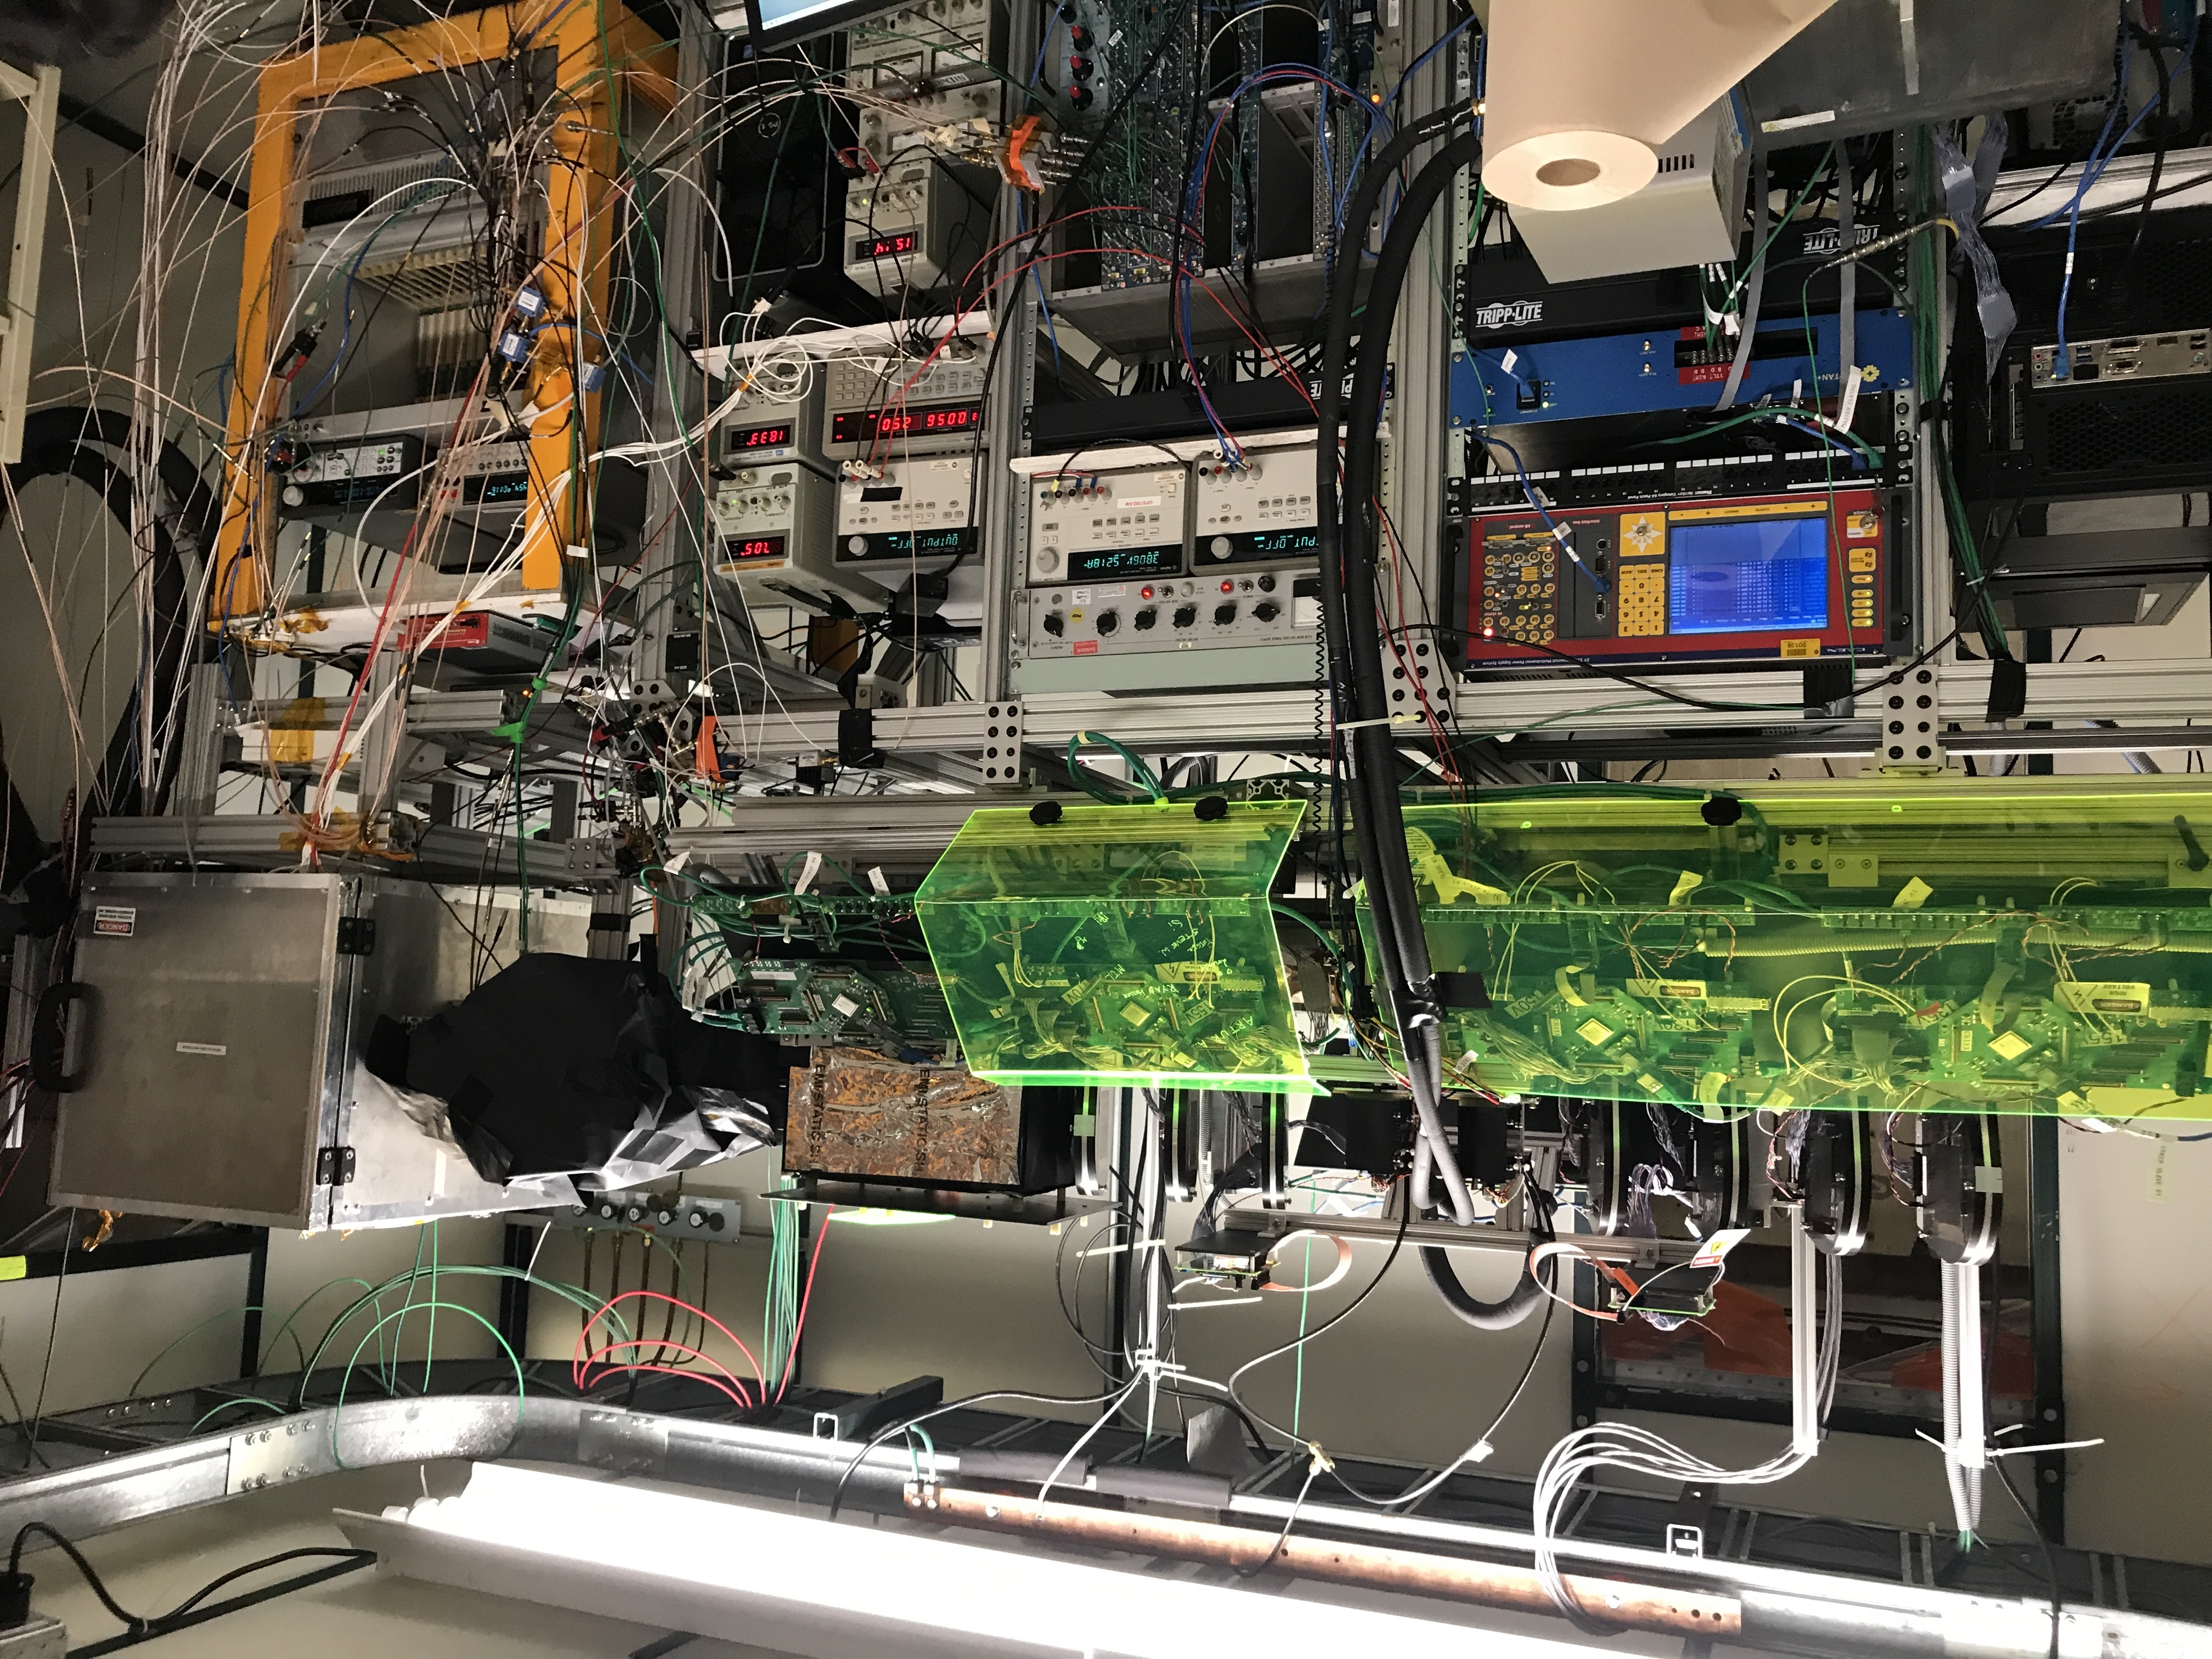
\includegraphics[width=0.8\textwidth,angle=180]{fig/ftbf_setup} 
\caption{A picture of the experimental area. The pixel telescope detectors are placed inside the 
electrostatic-discharge shielded boxes on the two sides of the DUT area. UPDATE DESCRIPTION} 
\label{fig:DragonBox} 
\end{figure} 


The beam is resonantly extracted in a slow spill for each Main Injector cycle
delivering a single 4.2 sec long spill per minute. The primary beam (bunched at
53 MHz) consists of 120~GeV protons. All measurements presented in this paper
were taken with the primary beam particles. The trigger to both the CAEN V1742
and to the pixel telescope was provided by a scintillator mounted on a
photomultiplier tube, placed upstream of the DUTs in the beam-line. Due to the
limited buffer depth of the CAEN V1742 board, special care had to be taken in
the design of the DAQ system to ensure that both the DUT and telescope DAQs
collect exactly the same amount of triggers. This was achieved by limiting the
trigger rate by introducing an adjustable dead-time using a custom-designed
trigger board. Processed data from the pixel telescope and the DUTs were
merged offline by matching the trigger counters recorded by the two systems.

\subsection{Readout Electronics}
This test beam makes use of two specialized readout boards: the single-channel UCSC board, optimized for time resolution measurements; and the 16-channel FNAL board, which enables simultanoues readout of many more channels.

The UCSC single-channel board is described in detail in
Ref.~\cite{Cartiglia201783}. This board uses discrete components and contains
several features which allow for maintaining a wide bandwidth ($\sim$ 2 GHz) and a
low noise even in noisy environments. The inverting amplifier uses a high-speed
SiGe transistor which has a transimpedance of about 470~$\Omega$. A commercial
inverting amplifier with gain 10x is used to boost the signal. The total transimpedance is 10.7.
k$\Omega$.

The 16-channel FNAL board is designed to test sensors up to 27~mm
by 15~mm at voltages up to 1~kV. Sixteen wire-bonding pads allow for signal readout via two stages of amplifiers based on Mini-Circuits GALI-66+. The amplifiers feature 25~$\Omega$ input impedance, 3.4~k$\Omega$ transimpedance, 1~GHz bandwidth, and approximately 1~mV rms output noise.

\section{Sensor radiation tolerance}
\label{sec:irradiationStudies}

% UFSD3 W5 - small sensors (1x3mm^2)
%   amplitude & time resolution vs irradiation
%   amplitude & time resolution vs BV
%   amplitude/time mean/time resolution vs position uniformity - 2D and 1D


\begin{figure}[htp] 
\centering 
\begin{tabular}{c} 
\includegraphics[width=0.79\textwidth]{fig/tP_VScan}  

\end{tabular} 
\caption{Time resolution as a function of bias voltage for three different irradiations.}
\label{fig:tp_VScan} 
\end{figure} 

\begin{figure}[htp] 
\centering 
\begin{tabular}{c} 
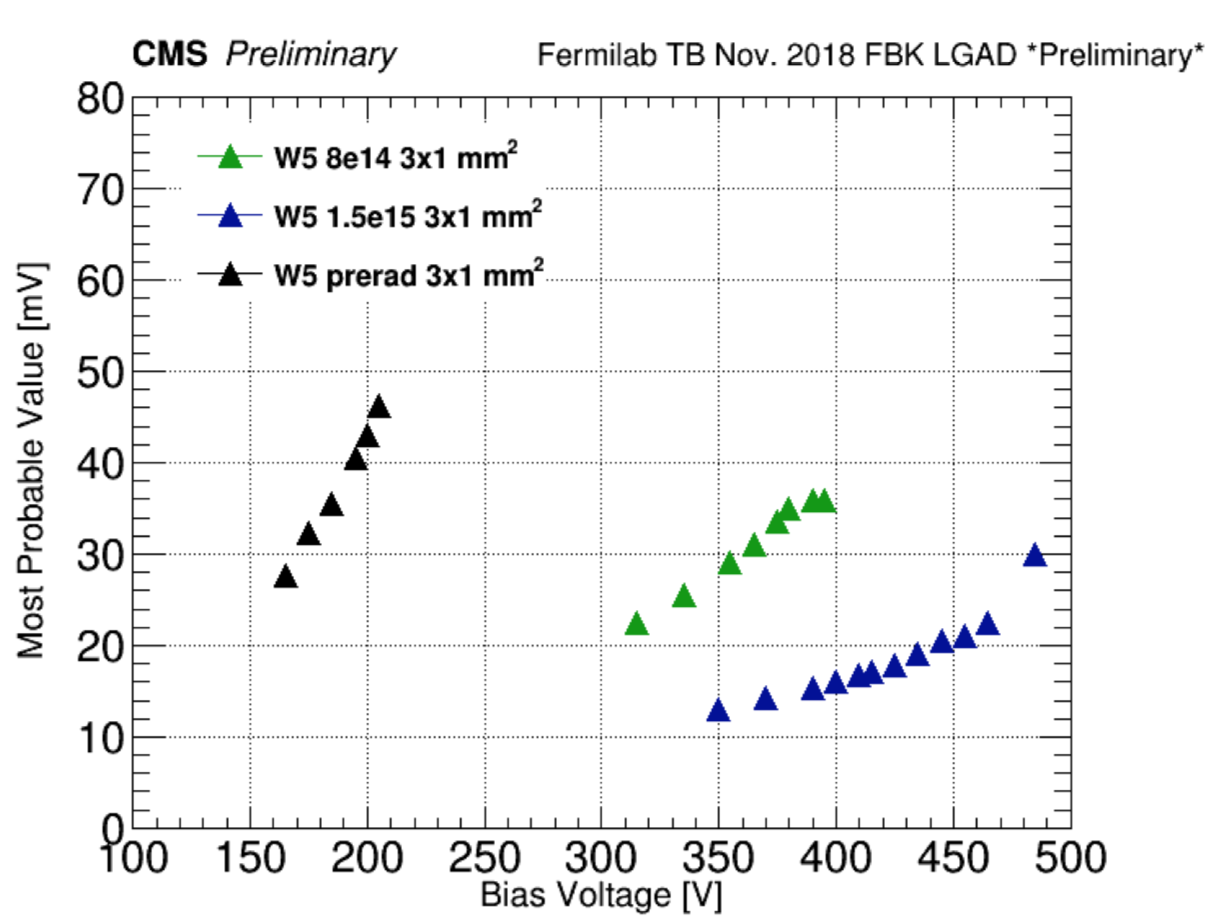
\includegraphics[width=0.49\textwidth]{fig/mpv_VScan}  
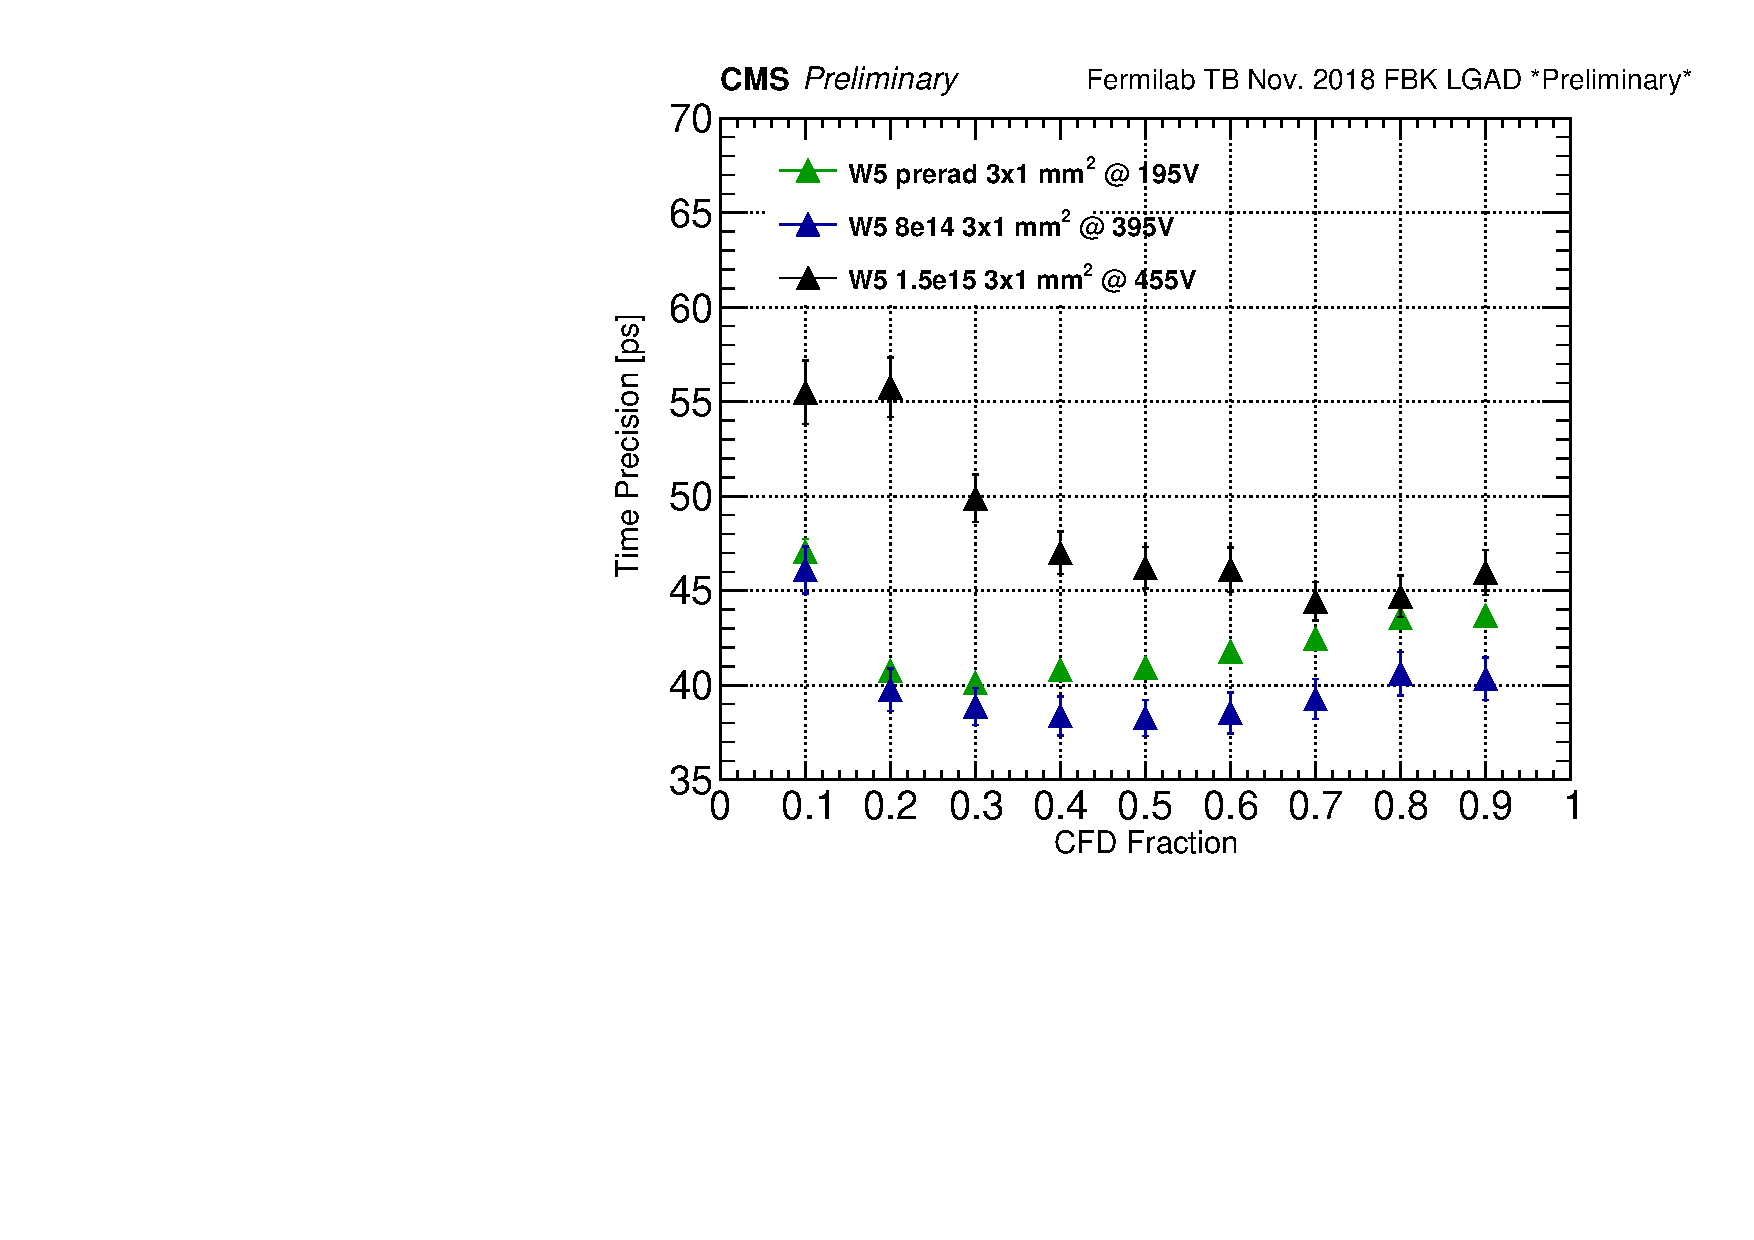
\includegraphics[width=0.49\textwidth]{fig/cfdScan}  

\end{tabular} 
\caption{Left: Gain as a function of bias voltage for three different irradiations. Right: Determination of optimum CFD threshold for example bias settings.}
\label{fig:gain_cfd_scan} 
\end{figure} 



\section{Uniformity of large area sensors}
\label{sec:largeAreaStudies}

% UFSD2 2x8 16-CH sensor - 
%   amplitude (& efficiency if we can get near 100%) vs position
%   time mean vs position - if we can take more data of this with Photek
%   Measurement of pixel gaps?

We present studies of the signal response across the active area of the FBK UFSD2 2x8 array. The hit efficiency as a function of x and y is shown in Fig ~\ref{fig:eff_map}. The efficiency is measured by taking the fraction of events with a signal above threshold (\SI{15}{\milli \volt}) out of all events with a high-quality track pointing towards the sensor. Events with more than one track or LGAD pad above threshold are removed from consideration, to avoid ambiguity in the proton position due to pileup or showering in upstream material.

The efficiency is observed to be highly uniform across the surface of the sensor, but with a constant apparent inefficiency of approximately 5-10\%. This inefficiency is not attributed to the sensor itself, but rather due to the occasional mismatch of events between the CAEN V1742 digitizer and the pixel telescope datastreams.

To isolate the sensor efficiency from the effects of synchronization loss, additional data was collected with a second LGAD sensor (HPK 50D-PIX from cite last paper) in front of the 2x8 array. Events with correct datastream matching are selected by requiring a track pointing to an HPK 50D channel, and a hit above threshold in that channel. Then, in this subset of events, the efficiency of the 2x8 array is measured for the channels in the shadow of the HPK sensor. The hit efficiency of the 2x8 array in this case is observed to be above 99\%. Based on the excellent uniformity of the sensor observed in the full dataset, it is reasonable to extrapolate that the true efficiency of the sensor is greater than 99\% for all channels.

\begin{figure}[htp] 
\centering {}
\begin{tabular}{c} 
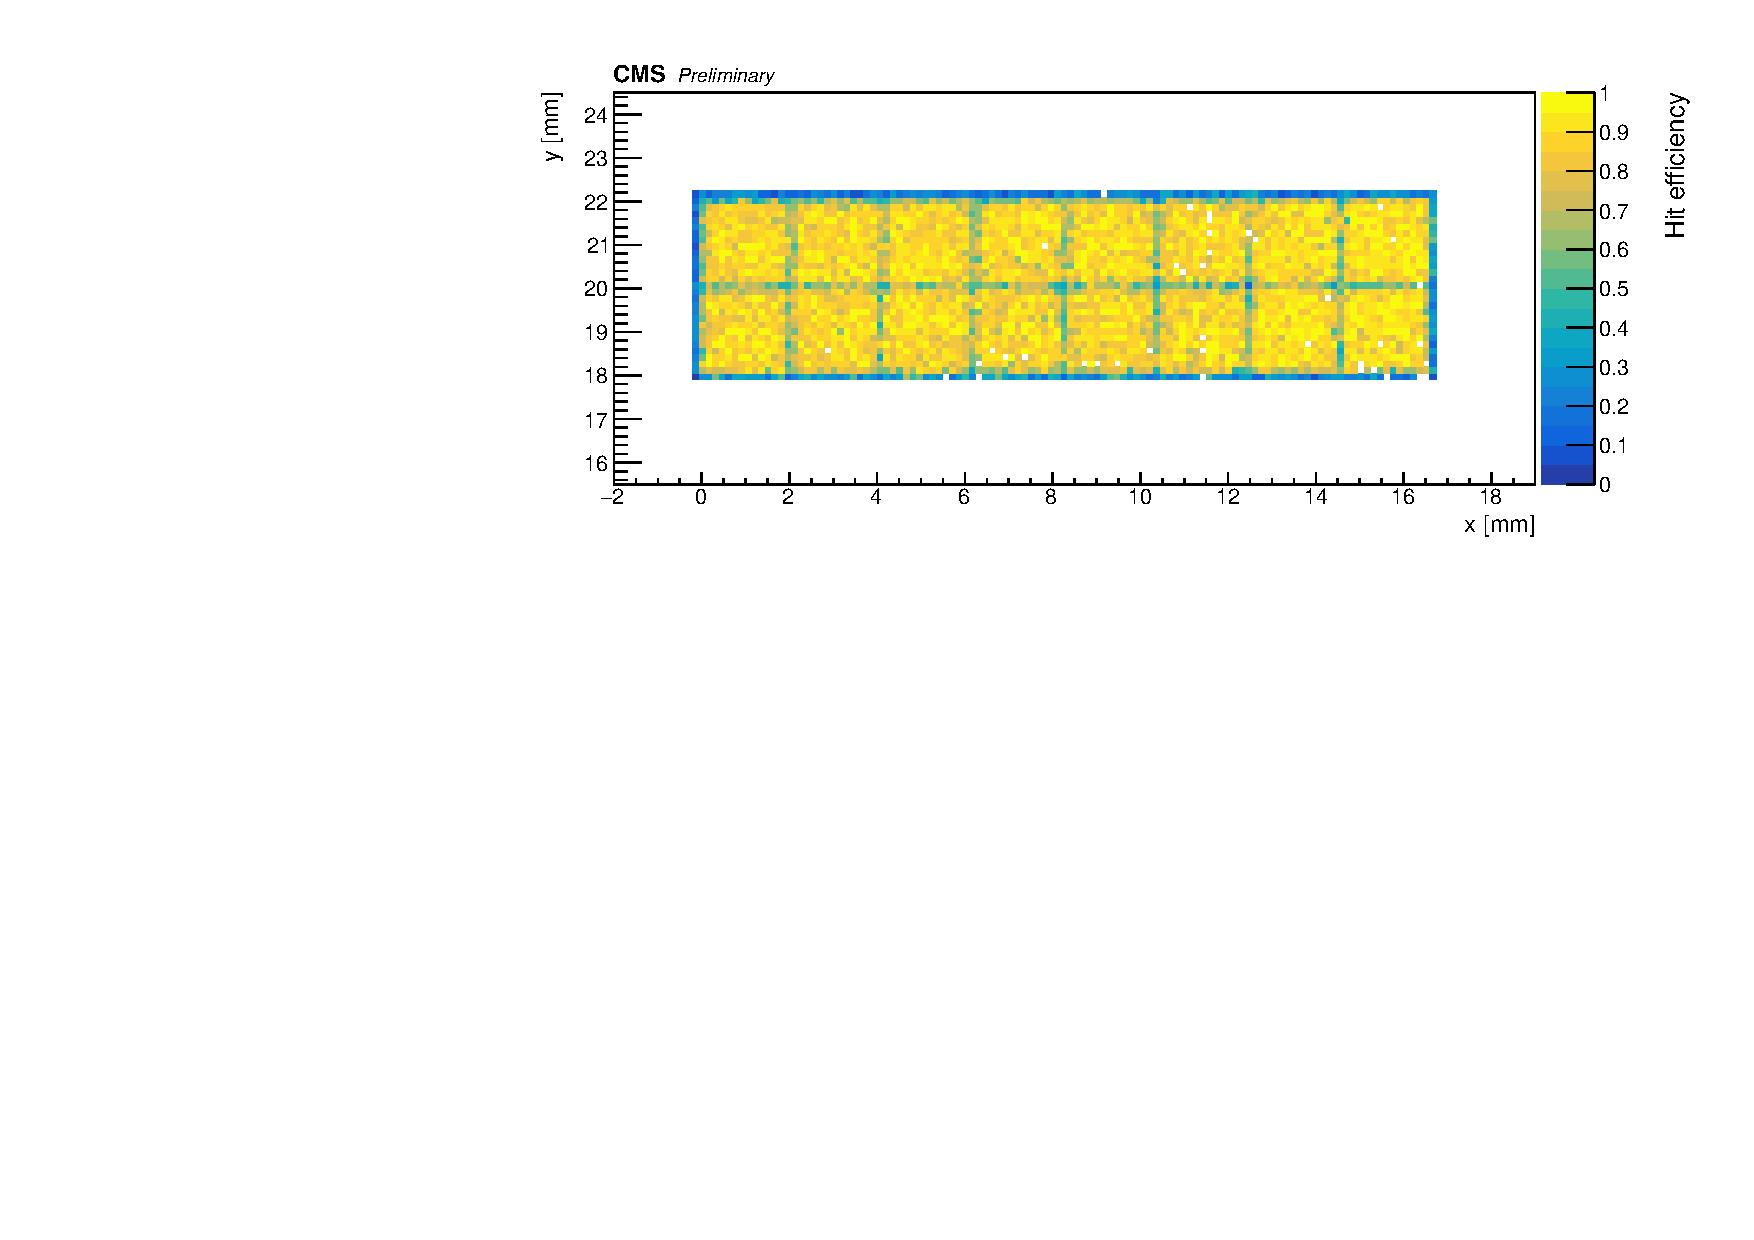
\includegraphics[width=0.99\textwidth]{fig/efficiency_map_unscaled}  
\end{tabular} 
\caption{Hit efficiency as a function of x and y across the sensor.} 
\label{fig:eff_map} 
\end{figure} 


Fig~\ref{fig:eff_map} shows typical signal amplitudes observed across the surface of the sensor. The amplitudes are quantified by extracting the most probable value from a Landau fit to the amplitude distributions for each position. A difference of approximately 15 \SI{15}{\milli\volt} is observed for different regions of the sensor, corresponding to a smooth gradient of approximately \SI{4}{\milli\volt \per \milli \meter}. The gradient does not correspond with any structure in the beam shape or temperature gradients in the sensor, and is present in data taken on separate occasions over several weeks. 

\begin{figure}[htp] 
\centering 
\begin{tabular}{c} 
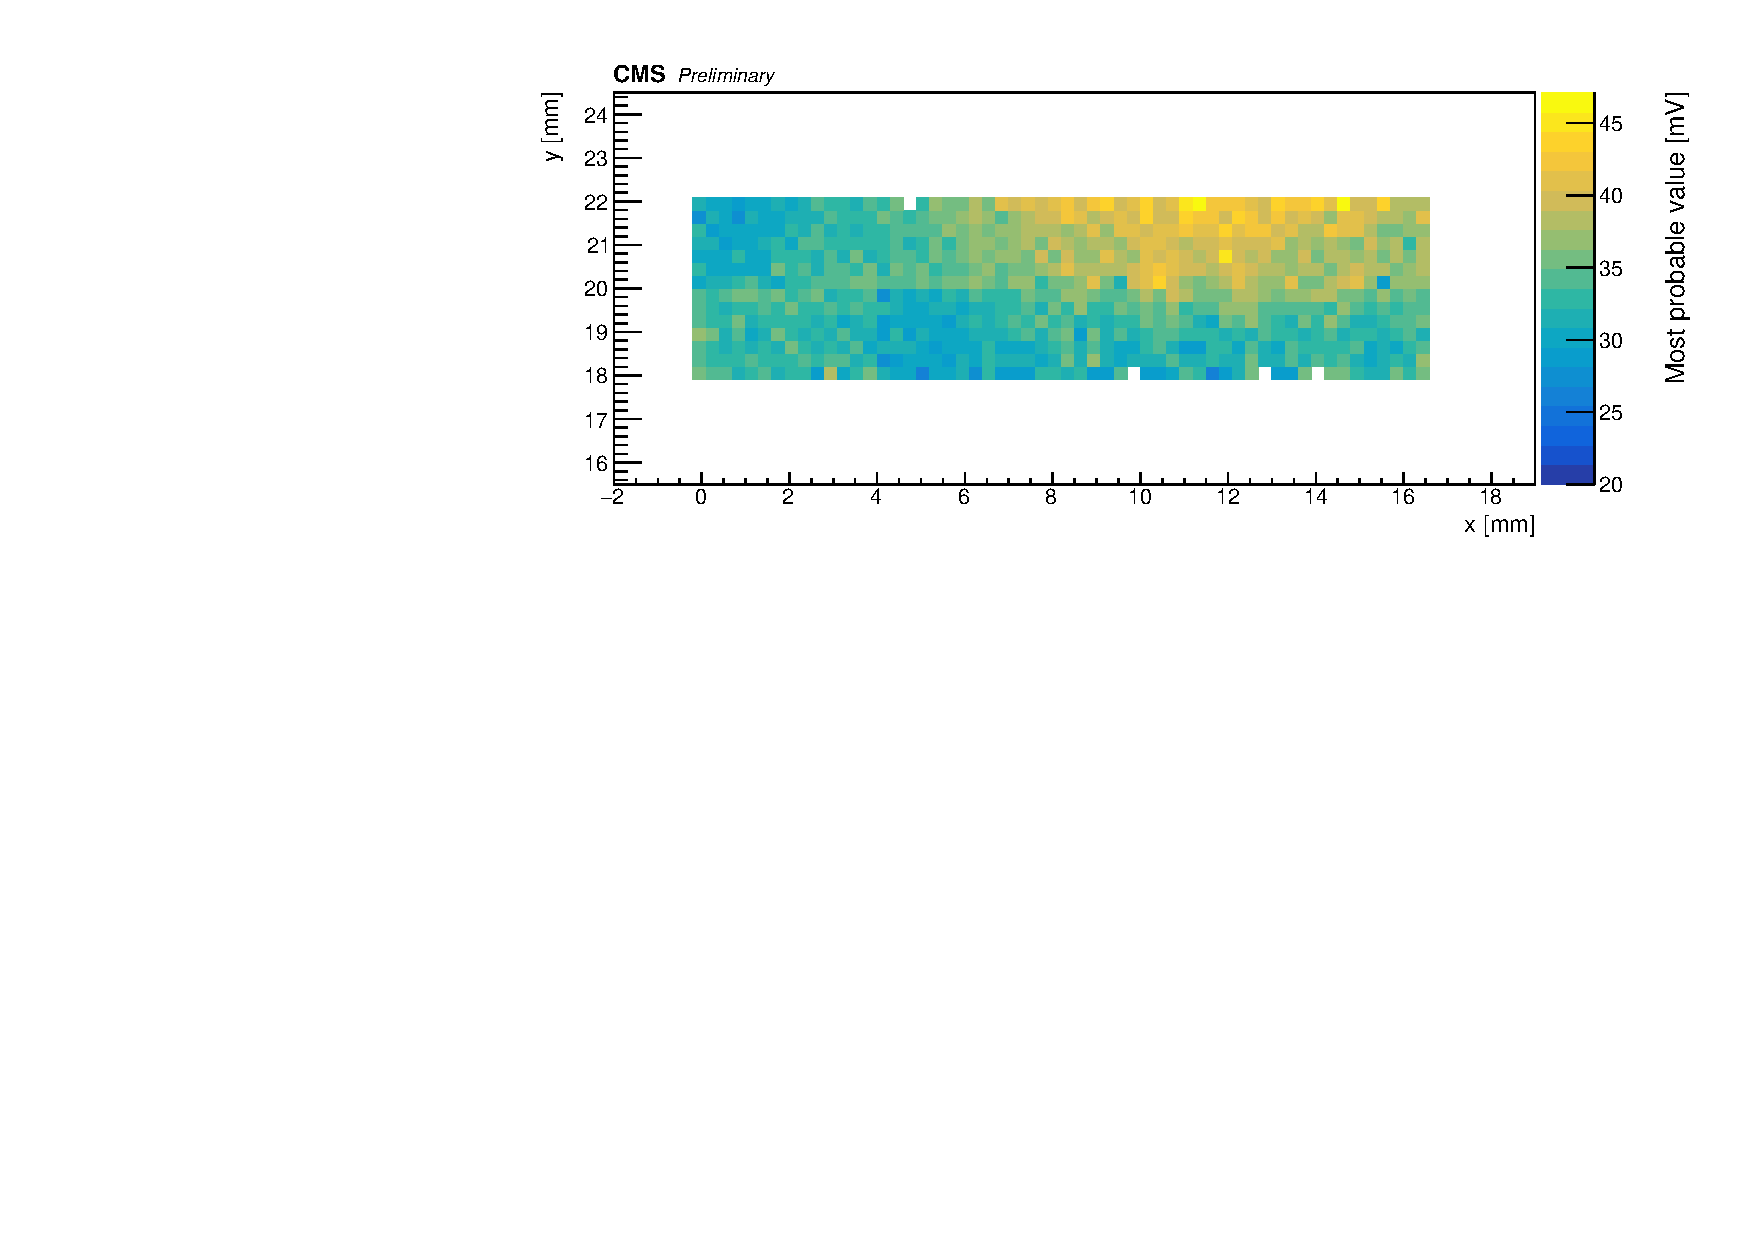
\includegraphics[width=0.99\textwidth]{fig/gain_map}  

\end{tabular} 
\caption{Most probable amplitude as a function of x and y across the sensor.} 
\label{fig:gain_map} 
\end{figure} 

 
\section{Conclusion}
\label{sec:conclusion} 


\section*{Acknowledgment}

We thank the FTBF personnel and Fermilab accelerator's team for very good beam
conditions during our test beam time. We also appreciate the technical support
of the Fermilab SiDet department for the rapid production of wire-bonded and
packaged LGAD assemblies. We would like to thank Alan Prosser and Ryan Rivera
for their critical help in setting up the DAQ and trigger chain. We thank Ned
Spencer, Max Wilder, and Forest McKinney-Martinez for their technical
assistance, and the CNM and HPK manufacturing team. We acknowledge the help of
V. Cindro and I. Mandic with the neutron irradiations. 

This document was prepared using the resources of the Fermi National Accelerator
Laboratory (Fermilab), a U.S. Department of Energy, Office of Science, HEP User
Facility. Fermilab is managed by Fermi Research Alliance, LLC (FRA), acting
under Contract No. DE-AC02-07CH11359. Part of this work was performed within the
framework of the CERN RD50 collaboration.

This work was supported by the Fermilab LDRD 2017.027; by the United States
Department of Energy grant DE-FG02-04ER41286; by the California Institute of
Technology High Energy Physics under Contract DE-SC0011925; by the European
Union's Horizon 2020 Research and Innovation funding program, under Grant
Agreement no. 654168 (AIDA-2020) and Grant Agreement no. 669529 (ERC
UFSD669529); by the Italian Ministero degli Affari Esteri and INFN Gruppo V; and
by the Spanish Ministry of Economy, Industry and Competitiveness through the
Particle Physics National Program (ref. FPA2014-55295-C3-2-R and
FPA2015-69260-C3-3-R) co-financed with FEDER funds.


% The Appendices part is started with the command \appendix;
% appendix sections are then done as normal sections

%\appendix
%\section{Appendix A}



% \section{}
% \label{}

%% If you have bibdatabase file and want bibtex to generate the
%% bibitems, please use
%%
%%  \bibliographystyle{elsarticle-num} 
%%  \bibliography{<your bibdatabase>}

%% else use the following coding to input the bibitems directly in the
%% TeX file.

\bibliography{LGAD_FBKUFSD3_FNALTB_Jan2019}{}
\bibliographystyle{ieeetr} 

%\begin{thebibliography}{00}

%% \bibitem{label}
%% Text of bibliographic item

%\bibitem{}

%\end{thebibliography}
\end{document}
\endinput
%%
%% End of file `elsarticle-template-num.tex'.


























